\documentclass[final]{beamer}
\usepackage[orientation=portrait,size=a1,scale=1.2]{beamerposter}
\usepackage[utf8]{inputenc}
\usepackage[T1]{fontenc}
\usepackage{lmodern}
\usepackage{amsmath,amssymb,mathtools}
\usepackage{booktabs}
\usepackage{makecell}
\usepackage{graphicx}
\usepackage{tikz}
\usepackage{pgfplots}
\pgfplotsset{compat=1.18}

\definecolor{ImperialBlue}{RGB}{0,0,205}
\definecolor{ImperialNavy}{RGB}{0,0,128}
\definecolor{LightBlueBg}{RGB}{230,238,255}

\usetheme{default}
\setbeamercolor{block title}{fg=white,bg=ImperialBlue}
\setbeamercolor{block body}{fg=black,bg=white}
\setbeamercolor{block alerted title}{fg=white,bg=ImperialNavy}
\setbeamercolor{block alerted body}{fg=black,bg=LightBlueBg}
\setbeamerfont{block title}{size=\large,series=\bfseries}
\setbeamerfont{block alerted title}{size=\large,series=\bfseries}
\setbeamerfont{block body}{size=\normalsize}
\setbeamertemplate{block begin}{
  \setbeamercolor{itemize item}{fg=ImperialBlue}
  \begin{beamercolorbox}[sep=0.8ex,colsep*=.5ex]{block title}
    \usebeamerfont{block title}\vphantom{Ayg}\insertblocktitle
  \end{beamercolorbox}
  {\parskip1ex\vskip-1ex}
  \begin{beamercolorbox}[colsep*=.75ex,sep=.75ex,vmode]{block body}
}
\setbeamertemplate{block end}{\end{beamercolorbox}\vskip1ex}
\setbeamertemplate{block alerted begin}{
  \begin{beamercolorbox}[sep=0.8ex,colsep*=.5ex]{block alerted title}
    \usebeamerfont{block alerted title}\vphantom{Ayg}\insertblocktitle
  \end{beamercolorbox}
  {\parskip1ex\vskip-1ex}
  \begin{beamercolorbox}[colsep*=.75ex,sep=.75ex,vmode]{block alerted body}
}
\setbeamertemplate{block alerted end}{\end{beamercolorbox}\vskip1ex}
\setbeamertemplate{navigation symbols}{}
\setbeamertemplate{itemize item}{\textcolor{ImperialBlue}{$\blacktriangleright$}}

\newcommand{\Om}{\Omega}
\newcommand{\Lp}[1]{L^{2}(#1)}
\newcommand{\Rmap}{\mathcal{R}}
\newcommand{\Jt}{\tilde{J}}

\title{}
\author{}
\date{}

\begin{document}
\begin{frame}[t]

\null\vspace*{0.5cm}

% ============= Header banner =============
\begin{beamercolorbox}[wd=\paperwidth,leftskip=1.5cm,rightskip=1.5cm]{block body}

\includegraphics[height=2cm, trim=55 105 52 105, clip]{figures/imperial_logo.png}\\[0.3em]
{\color{ImperialBlue}\rule{\dimexpr\paperwidth-3cm\relax}{2pt}}\\[0.6em]
\begin{minipage}[t]{0.68\dimexpr\paperwidth-3cm\relax}
{\color{ImperialBlue}\LARGE\bfseries
Mesh Dependence in PDE-Constrained Optimisation \\
with Firedrake, pyadjoint, and PETSc TAO}\\[0.2em]
{\color{ImperialBlue}\large
Reproducing Schwedes' iteration-count benchmark and extending it to the inner Krylov solve}
\end{minipage}%
\hfill
\begin{minipage}[t]{0.28\dimexpr\paperwidth-3cm\relax}
\raggedright
{\color{ImperialBlue}\normalsize\bfseries
Bert Jim Chang\\
Supervisor: David A.\ Ham\\
Department of Mathematics}
\end{minipage}\\[0.4em]
{\color{ImperialBlue}\rule{\dimexpr\paperwidth-3cm\relax}{1pt}}
\end{beamercolorbox}

\vspace{0.1cm}

% ============= Two-column body =============
\begin{columns}[t,totalwidth=\dimexpr\paperwidth-3cm\relax]

% ============= LEFT COLUMN =============
\begin{column}{0.49\dimexpr\paperwidth-3cm\relax}

\begin{block}{Context}
Firedrake is an open-source finite element library, and \texttt{pyadjoint} is its adjoint extension for optimisation. Together they let a user write a PDE-constrained optimisation problem in near-mathematical syntax and have it solved automatically.

The library currently supports several optimisation backends: SciPy for general use, ROL as the backend for the Fireshape shape-optimisation toolkit, and PETSc TAO as a more recent option that recent Firedrake demos point at for parallel workloads. For this direction to hold up, TAO has to be shown to behave correctly on the kind of problem Firedrake users actually solve: one where the control is a \emph{function} on a domain rather than a vector of numbers, and where the natural way to measure angle and distance on the control space is a Hilbert-space inner product rather than the standard Euclidean one.
\end{block}

\begin{block}{The mesh-dependence phenomenon}
Schwedes et al.\ (2017) show that gradient-based optimisation over a Hilbert function space is mesh-independent if and only if the algorithm respects that space's inner product. Their \emph{iteration-count benchmark} makes the effect empirically visible: the same Poisson optimal control problem is solved on a sequence of increasingly non-uniformly refined meshes, and the number of outer iterations each optimiser takes to converge is recorded. Optimisers hard-coded to the Euclidean $\ell^{2}$ inner product produce iteration counts that grow polynomially with mesh refinement, while ones using the natural $L^{2}$ inner product stay flat.

The fix runs through a single operator, the \emph{Riesz map}. It converts a functional's derivative (which naturally sits in the dual space $H^{*}$) into an element of $H$ that the optimiser can use as a search direction. In the discrete $L^{2}$ setting,
\[
\Rmap_{L^{2}} \;=\; M_{h}^{-1},
\]
the inverse of the assembled Galerkin mass matrix. Skipping this step leaves the mesh-scaling factor in $M_{h}$ uncancelled, which produces the polynomial growth on non-uniformly refined meshes.
\end{block}

\begin{block}{Test problem and setup}
Poisson optimal control: find a source term $m \in \Lp{\Om}$ that minimises
\[
\Jt(m) = \tfrac{1}{2}\|u-d\|_{\Lp{\Om}}^{2} + \tfrac{\alpha}{2}\|m\|_{\Lp{\Om}}^{2},
\quad
\text{s.t.} \quad -\Delta u = m \text{ on } \Om,\ u = 0 \text{ on } \partial\Om,
\]
on $\Om = (0,1)^{2}$ with desired state $d = \sin(\pi x)\sin(\pi y)$ and regularisation $\alpha = 10^{-4}$. The reduced gradient is derived by hand using the adjoint method and computed at run time using \texttt{pyadjoint}, which records a tape of the forward solve and plays it back in reverse. Verification is by a manufactured-solution convergence test and by a Taylor test on the reduced gradient, both showing second-order behaviour.

The mesh sequence follows Schwedes et al.\ (2017, Sect.~2.3.2.1) exactly: starting from a uniform $8\times 8$ triangulation of the unit square, at each level every cell is independently marked with probability $p = 0.35$ and Rivara-bisected on its longest edge, with LEPP chain propagation keeping the mesh conforming. Refinement scatters through the interior, so the Dirichlet boundary is treated symmetrically. Realised $h_{\max}/h_{\min}$ grows from $1$ to $\sim 5.7$ across levels 0--10.

\vspace{0.4cm}
\begin{minipage}{0.48\linewidth}
\centering
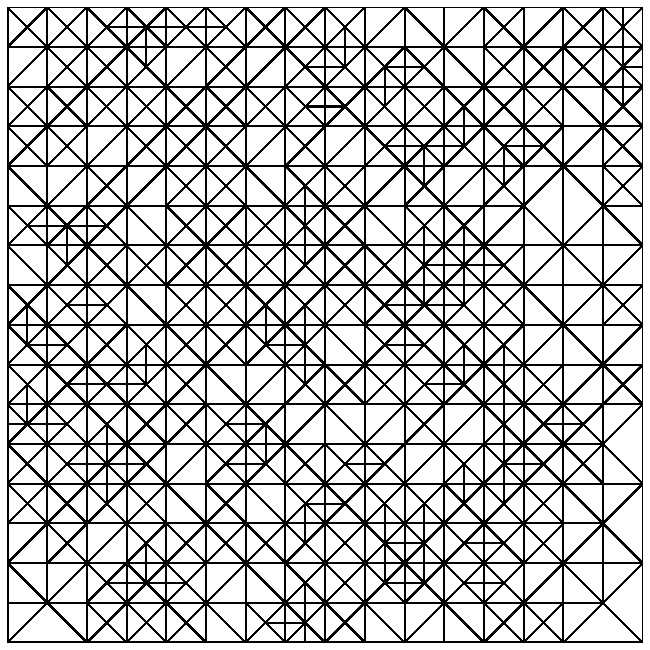
\includegraphics[width=\linewidth]{figures/random_mesh_level4.pdf}\\[0.2em]
{\small Level 4 ($1027$ cells, ratio $2.8$)}
\end{minipage}%
\hfill
\begin{minipage}{0.48\linewidth}
\centering
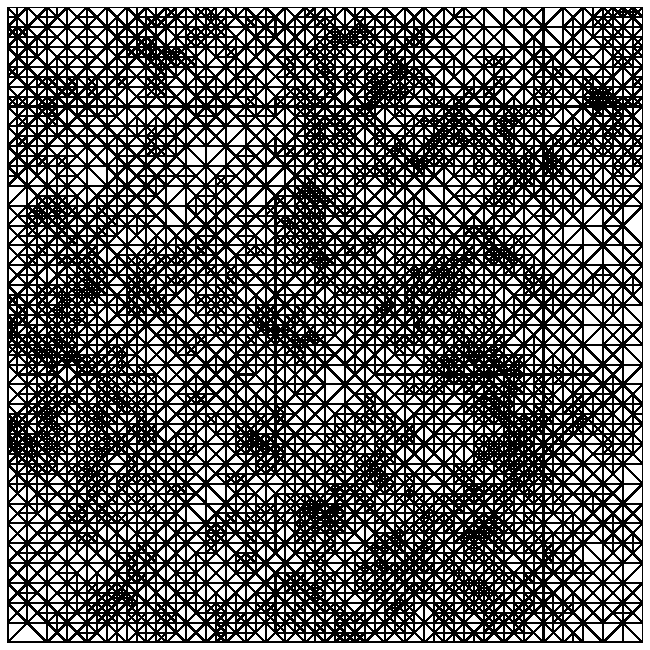
\includegraphics[width=\linewidth]{figures/random_mesh_level8.pdf}\\[0.2em]
{\small Level 8 ($9670$ cells, ratio $5.7$)}
\end{minipage}
\end{block}

\end{column}

% ============= RIGHT COLUMN =============
\begin{column}{0.49\dimexpr\paperwidth-3cm\relax}

\begin{block}{Objectives}
\begin{enumerate}
\item \textbf{Show that TAO works correctly at the outer level.} Reproduce Schwedes' iteration-count benchmark in the Firedrake + \texttt{pyadjoint} + TAO stack. Find the settings that make TAO's \texttt{lmvm} solver match the flat row. Test the other TAO solvers (\texttt{nls}, \texttt{bqnls}, \texttt{cg}) to see which inherit the good behaviour and which do not.
\item \textbf{Fix the mesh-dependence at the inner solver level.} TAO's \texttt{nls} solver takes only two outer Newton iterations because the Poisson problem is quadratic. Each Newton step, however, solves a linear system with an inner CG whose iteration count the outer table does not show. Show that this inner count grows with mesh grading and that an $L^{2}$ Riesz-map preconditioner fixes it. This is the piece Schwedes does not test.
\item \textbf{Work out the pyadjoint interface.} Determine how the \texttt{TAOSolver} wrapper should expose the Riesz-map mechanism so end users get correct mesh-independent behaviour by default.
\end{enumerate}
\end{block}

\begin{block}{Reproducing the experiment (outer L-BFGS)}
Both L-BFGS optimisers were run to $\|\Rmap_{L^{2}}(J')\|_{\Lp{\Om}} \le 10^{-7}$ across six refinement levels. The reference implementation is a hand-written Hilbert-space L-BFGS following Schwedes et al.\ (2017, Sect.~1.5.4.1); the SciPy row is \texttt{L-BFGS-B} in $\ell^{2}$ with the convergence check done externally in $L^{2}$.

\vspace{0.3em}
\centering
\begin{tabular}{lrrrrrr}
\toprule
Optimiser (inner product used) & L=0 & L=2 & L=4 & L=6 & L=8 & L=10 \\
\midrule
SciPy \texttt{L-BFGS-B} ($\ell^{2}$)          & 13 & 31 & 35 & 47 & 47 & 55 \\
Hand-written Hilbert L-BFGS ($L^{2}$)         &  6 &  8 &  6 &  6 &  5 &  4 \\
\bottomrule
\end{tabular}

\vspace{0.4em}
\raggedright
Cell counts across the sweep: $128, 340, 1027, 3174, 9670, 29474$. Realised $h_{\max}/h_{\min}$: $1.00, 2.00, 2.83, 4.00, 5.66, 5.66$. The SciPy $\ell^{2}$ row grows roughly $4\times$ across the sweep; the Hilbert $L^{2}$ row stays flat between 4 and 8 iterations. TAO's \texttt{lmvm} reproduces the flat row once its default history length of five is raised to 100.
\end{block}

\begin{alertblock}{New result: preconditioning the inner CG of TAO/NLS}
TAO/NLS converges in two outer Newton steps at every mesh (the Poisson problem is quadratic in $m$). The total \emph{inner-CG} count across those two steps, however, grows with refinement. Attaching an $L^{2}$ Riesz-map preconditioner to the inner KSP, using a plain PETSc Python PC (\texttt{RieszMapPCContext}) that assembles $M_{h}$ once and applies $M_{h}^{-1}$ on every inner call, restores mesh-independence.

\vspace{0.3em}
\centering
\begin{tikzpicture}
\begin{axis}[
  width=0.95\linewidth, height=8.5cm,
  xlabel={Refinement level},
  ylabel={Total inner-CG iterations\\across both Newton steps},
  ylabel style={align=center},
  xtick={0,2,4,6,8,10},
  ymin=0, ymax=85,
  grid=major,
  legend pos=north west,
  legend style={font=\small,draw=none,fill=none},
  every axis plot/.append style={line width=1.2pt, mark size=3.5pt},
]
\addplot[color=red!80!black, mark=*]
  coordinates {(0,24) (2,39) (4,45) (6,50) (8,61) (10,73)};
\addlegendentry{TAO/NLS, no preconditioner}
\addplot[color=ImperialBlue, mark=square*]
  coordinates {(0,10) (2,14) (4,14) (6,13) (8,13) (10,12)};
\addlegendentry{TAO/NLS + $M_h^{-1}$ inner PC}
\end{axis}
\end{tikzpicture}

\vspace{0.2em}
\raggedright\small
Baseline inner-CG counts grow from 24 to 73 across the sweep (levels 0 to 10, up to 29\,474 cells). With the $L^{2}$ Riesz-map preconditioner installed on TAO's inner KSP, the count stays between 10 and 14 across the whole sweep. This is the outer-optimiser argument carried down to the inner Krylov solve, and it is what Schwedes et al.\ (2017, Sect.~1.3.3) points at via Kirby (2010) but does not test experimentally.
\end{alertblock}

\begin{block}{Work plan for the remaining time}
\begin{itemize}
\item \textbf{Diagnose \texttt{bqnls}'s line search.} Rerun the mesh sweep with \texttt{tao\_ls\_monitor} to distinguish a history-size issue (as with stock \texttt{lmvm}) from a projected line-search bug.
\item \textbf{$H^{1}$ Riesz preconditioner sweep.} The preconditioner module already handles the $H^{1}$ form. Adding an $H^{1}$ column to the inner-CG table would round off the story symmetrically with Schwedes' $H^{1}$ variant of the benchmark.
\item \textbf{Interface design writeup.} Draft a short document laying out how the \texttt{TAOSolver} wrapper should expose the Riesz-map mechanism to users.
\end{itemize}
\end{block}

\begin{block}{References}
\footnotesize
\begin{itemize}\itemsep0.1em
\item Schwedes, Ham, Funke, Piggott (2017). \textit{Mesh Dependence in PDE-Constrained Optimisation}. SpringerBriefs.
\item Kirby (2010). From functional analysis to iterative methods. \textit{SIAM Review} 52(2).
\item Rathgeber et al.\ (2016). Firedrake: automating the finite element method. \textit{ACM TOMS} 43(3).
\item Mitusch, Funke, Dokken (2019). dolfin-adjoint 2018.1. \textit{JOSS} 4(38).
\item Sch{\"o}berl (1997). NETGEN: an advancing-front 2D/3D mesh generator. \textit{Comput.\ Vis.\ Sci.} 1(1).
\end{itemize}
\end{block}

\end{column}

\end{columns}

% ============= Footer =============
\vfill
\begin{beamercolorbox}[wd=\paperwidth,leftskip=1.5cm,rightskip=1.5cm]{block body}
{\color{ImperialBlue}\rule{\dimexpr\paperwidth-3cm\relax}{1pt}}\\[0.2em]
\hbox to \dimexpr\paperwidth-3cm\relax{%
  {\color{ImperialBlue}\normalsize Imperial College London}%
  \hfill
  {\color{ImperialBlue}\normalsize MSc Summer Research Fair, July 2026}%
  \hfill
  {\color{ImperialBlue}\normalsize imperial.ac.uk}%
}
\end{beamercolorbox}

\end{frame}
\end{document}
